
\documentclass[a4paper,11pt]{article}
\usepackage[a4paper, margin=8em]{geometry}

% usa i pacchetti per la scrittura in italiano
\usepackage[french,italian]{babel}
\usepackage[T1]{fontenc}
\usepackage[utf8]{inputenc}
\frenchspacing 

% usa i pacchetti per la formattazione matematica
\usepackage{amsmath, amssymb, amsthm, amsfonts}

% usa altri pacchetti
\usepackage{gensymb}
\usepackage{hyperref}
\usepackage{standalone}

\usepackage{colortbl}

\usepackage{xstring}
\usepackage{karnaugh-map}

% imposta il titolo
\title{Appunti Calcolatori Elettronici}
\author{Luca Seggiani}
\date{2025}

% imposta lo stile
% usa helvetica
\usepackage[scaled]{helvet}
% usa palatino
\usepackage{palatino}
% usa un font monospazio guardabile
\usepackage{lmodern}

\renewcommand{\rmdefault}{ppl}
\renewcommand{\sfdefault}{phv}
\renewcommand{\ttdefault}{lmtt}

% circuiti
\usepackage{circuitikz}
\usetikzlibrary{babel}

% testo cerchiato
\newcommand*\circled[1]{\tikz[baseline=(char.base)]{
            \node[shape=circle,draw,inner sep=2pt] (char) {#1};}}

% disponi il titolo
\makeatletter
\renewcommand{\maketitle} {
	\begin{center} 
		\begin{minipage}[t]{.8\textwidth}
			\textsf{\huge\bfseries \@title} 
		\end{minipage}%
		\begin{minipage}[t]{.2\textwidth}
			\raggedleft \vspace{-1.65em}
			\textsf{\small \@author} \vfill
			\textsf{\small \@date}
		\end{minipage}
		\par
	\end{center}

	\thispagestyle{empty}
	\pagestyle{fancy}
}
\makeatother

% disponi teoremi
\usepackage{tcolorbox}
\newtcolorbox[auto counter, number within=section]{theorem}[2][]{%
	colback=blue!10, 
	colframe=blue!40!black, 
	sharp corners=northwest,
	fonttitle=\sffamily\bfseries, 
	title=Teorema~\thetcbcounter: #2, 
	#1
}

% disponi definizioni
\newtcolorbox[auto counter, number within=section]{definition}[2][]{%
	colback=red!10,
	colframe=red!40!black,
	sharp corners=northwest,
	fonttitle=\sffamily\bfseries,
	title=Definizione~\thetcbcounter: #2,
	#1
}

% disponi codice
\usepackage{listings}
\usepackage[table]{xcolor}

\definecolor{codegreen}{rgb}{0,0.6,0}
\definecolor{codegray}{rgb}{0.5,0.5,0.5}
\definecolor{codepurple}{rgb}{0.58,0,0.82}
\definecolor{backcolour}{rgb}{0.95,0.95,0.92}

\lstdefinestyle{codestyle}{
		backgroundcolor=\color{black!5}, 
		commentstyle=\color{codegreen},
		keywordstyle=\bfseries\color{magenta},
		numberstyle=\sffamily\tiny\color{black!60},
		stringstyle=\color{green!50!black},
		basicstyle=\ttfamily\footnotesize,
		breakatwhitespace=false,         
		breaklines=true,                 
		captionpos=b,                    
		keepspaces=true,                 
		numbers=left,                    
		numbersep=5pt,                  
		showspaces=false,                
		showstringspaces=false,
		showtabs=false,                  
		tabsize=2
}

\lstdefinestyle{shellstyle}{
		backgroundcolor=\color{black!5}, 
		basicstyle=\ttfamily\footnotesize\color{black}, 
		commentstyle=\color{black}, 
		keywordstyle=\color{black},
		numberstyle=\color{black!5},
		stringstyle=\color{black}, 
		showspaces=false,
		showstringspaces=false, 
		showtabs=false, 
		tabsize=2, 
		numbers=none, 
		breaklines=true
}


\lstdefinelanguage{assembler}{ 
  keywords={AAA, AAD, AAM, AAS, ADC, ADCB, ADCW, ADCL, ADD, ADDB, ADDW, ADDL, AND, ANDB, ANDW, ANDL,
        ARPL, BOUND, BSF, BSFL, BSFW, BSR, BSRL, BSRW, BSWAP, BT, BTC, BTCB, BTCW, BTCL, BTR, 
        BTRB, BTRW, BTRL, BTS, BTSB, BTSW, BTSL, CALL, CBW, CDQ, CLC, CLD, CLI, CLTS, CMC, CMP,
        CMPB, CMPW, CMPL, CMPS, CMPSB, CMPSD, CMPSW, CMPXCHG, CMPXCHGB, CMPXCHGW, CMPXCHGL,
        CMPXCHG8B, CPUID, CWDE, DAA, DAS, DEC, DECB, DECW, DECL, DIV, DIVB, DIVW, DIVL, ENTER,
        HLT, IDIV, IDIVB, IDIVW, IDIVL, IMUL, IMULB, IMULW, IMULL, IN, INB, INW, INL, INC, INCB,
        INCW, INCL, INS, INSB, INSD, INSW, INT, INT3, INTO, INVD, INVLPG, IRET, IRETD, JA, JAE,
        JB, JBE, JC, JCXZ, JE, JECXZ, JG, JGE, JL, JLE, JMP, JNA, JNAE, JNB, JNBE, JNC, JNE, JNG,
        JNGE, JNL, JNLE, JNO, JNP, JNS, JNZ, JO, JP, JPE, JPO, JS, JZ, LAHF, LAR, LCALL, LDS,
        LEA, LEAVE, LES, LFS, LGDT, LGS, LIDT, LMSW, LOCK, LODSB, LODSD, LODSW, LOOP, LOOPE,
        LOOPNE, LSL, LSS, LTR, MOV, MOVB, MOVW, MOVL, MOVSB, MOVSD, MOVSW, MOVSX, MOVSXB,
        MOVSXW, MOVSXL, MOVZX, MOVZXB, MOVZXW, MOVZXL, MUL, MULB, MULW, MULL, NEG, NEGB, NEGW,
        NEGL, NOP, NOT, NOTB, NOTW, NOTL, OR, ORB, ORW, ORL, OUT, OUTB, OUTW, OUTL, OUTSB, OUTSD,
        OUTSW, POP, POPL, POPW, POPB, POPA, POPAD, POPF, POPFD, PUSH, PUSHL, PUSHW, PUSHB, PUSHA, 
				PUSHAD, PUSHF, PUSHFD, RCL, RCLB, RCLW, MOVSL, MOVSB, MOVSW, STOSL, STOSB, STOSW, LODSB, LODSW,
				LODSL, INSB, INSW, INSL, OUTSB, OUTSL, OUTSW
        RCLL, RCR, RCRB, RCRW, RCRL, RDMSR, RDPMC, RDTSC, REP, REPE, REPNE, RET, ROL, ROLB, ROLW,
        ROLL, ROR, RORB, RORW, RORL, SAHF, SAL, SALB, SALW, SALL, SAR, SARB, SARW, SARL, SBB,
        SBBB, SBBW, SBBL, SCASB, SCASD, SCASW, SETA, SETAE, SETB, SETBE, SETC, SETE, SETG, SETGE,
        SETL, SETLE, SETNA, SETNAE, SETNB, SETNBE, SETNC, SETNE, SETNG, SETNGE, SETNL, SETNLE,
        SETNO, SETNP, SETNS, SETNZ, SETO, SETP, SETPE, SETPO, SETS, SETZ, SGDT, SHL, SHLB, SHLW,
        SHLL, SHLD, SHR, SHRB, SHRW, SHRL, SHRD, SIDT, SLDT, SMSW, STC, STD, STI, STOSB, STOSD,
        STOSW, STR, SUB, SUBB, SUBW, SUBL, TEST, TESTB, TESTW, TESTL, VERR, VERW, WAIT, WBINVD,
        XADD, XADDB, XADDW, XADDL, XCHG, XCHGB, XCHGW, XCHGL, XLAT, XLATB, XOR, XORB, XORW, XORL},
  keywordstyle=\color{blue}\bfseries,
  ndkeywordstyle=\color{darkgray}\bfseries,
  identifierstyle=\color{black},
  sensitive=false,
  comment=[l]{\#},
  morecomment=[s]{/*}{*/},
  commentstyle=\color{purple}\ttfamily,
  stringstyle=\color{red}\ttfamily,
  morestring=[b]',
  morestring=[b]"
}

\lstset{language=assembler, style=codestyle}

% disponi sezioni
\usepackage{titlesec}

\titleformat{\section}
	{\sffamily\Large\bfseries} 
	{\thesection}{1em}{} 
\titleformat{\subsection}
	{\sffamily\large\bfseries}   
	{\thesubsection}{1em}{} 
\titleformat{\subsubsection}
	{\sffamily\normalsize\bfseries} 
	{\thesubsubsection}{1em}{}

% tikz
\usepackage{tikz}

% float
\usepackage{float}

% grafici
\usepackage{pgfplots}
\pgfplotsset{width=10cm,compat=1.9}

% disponi alberi
\usepackage{forest}

\forestset{
	rectstyle/.style={
		for tree={rectangle,draw,font=\large\sffamily}
	},
	roundstyle/.style={
		for tree={circle,draw,font=\large}
	}
}

% disponi algoritmi
\usepackage{algorithm}
\usepackage{algorithmic}
\makeatletter
\renewcommand{\ALG@name}{Algoritmo}
\makeatother

% disponi numeri di pagina
\usepackage{fancyhdr}
\fancyhf{} 
\fancyfoot[L]{\sffamily{\thepage}}

\makeatletter
\fancyhead[L]{\raisebox{1ex}[0pt][0pt]{\sffamily{\@title \ \@date}}} 
\fancyhead[R]{\raisebox{1ex}[0pt][0pt]{\sffamily{\@author}}}
\makeatother

\begin{document}
% sezione (data)
\section{Lezione del 07-03-25}

% stili pagina
\thispagestyle{empty}
\pagestyle{fancy}

% testo
Riprendiamo il discorso della memoria cache.

\subsubsection{Cache e I/O}
Avevamo che la memoria cache è montata fra la CPU e lo spazio di memoria: più propriamente, si trova fra la CPU e il bus.
Può quindi vedere non solo le operazioni sulla memoria, ma anche sullo spazio di I/O.
In questo caso, però, dovrà ovviamente comportarsi sempre in maniera \textit{read-through} e \textit{write-through}, quindi effettivamente disattivarsi e lasciare che il processore interagisca direttamente con l'I/O.

Questo è dovuto al fatto che allo spazio di I/O potrebbero accedere e modificare dati dispositivi esterni alla CPU (le interfacce), operazione che invaliderebbe immediatamente qualsiasi cosa venga scritta in memoria cache.

Inoltre, ogni operazione di lettura può comportare di per sé un aggiornamento delle interfacce, che comporterà un aggiornamento della memoria, motivo per cui un operazione di caching sarebbe superflua se non addirittura dannosa.

Operazione simile varrà effettuata per la memoria video (che non sta nello spazio di I/O).
Questa facoltà verra realizzata dalla cache attraverso, probabilmente, \textit{maschere} o \textit{tabelle} che tengono conto di dove si trova la memoria video, e quindi quali richieste di lettura e scrittura vi hanno luogo.

\subsubsection{Cache associative ad insiemi}
Avevamo visto come il difetto principale della cache ad indirizzamento diretta è quello delle \textit{collisioni}.
Presentiamo un metodo, quello delle \textbf{cache associative ad insiemi}, che risolve il problema permettendo di allocare più cacheline allo stesso indirizzo.

Duplichiamo quindi la struttura vista per la cache ad indirizzamento diretto (qui solo 1 volta, anche se nei sistemi moderni si va dai 4-8 insiemi per le cache di primo livello e 8-16 insiemi per le cache di secondo e terzo livello), e sfruttiamo le uscite hit/miss delle singole memorie delle etichette per pilotare un multiplexer con in ingresso le linee dati delle memorie di cache corrispondenti.

La struttura così modificata sarà la seguente:
\begin{center}
	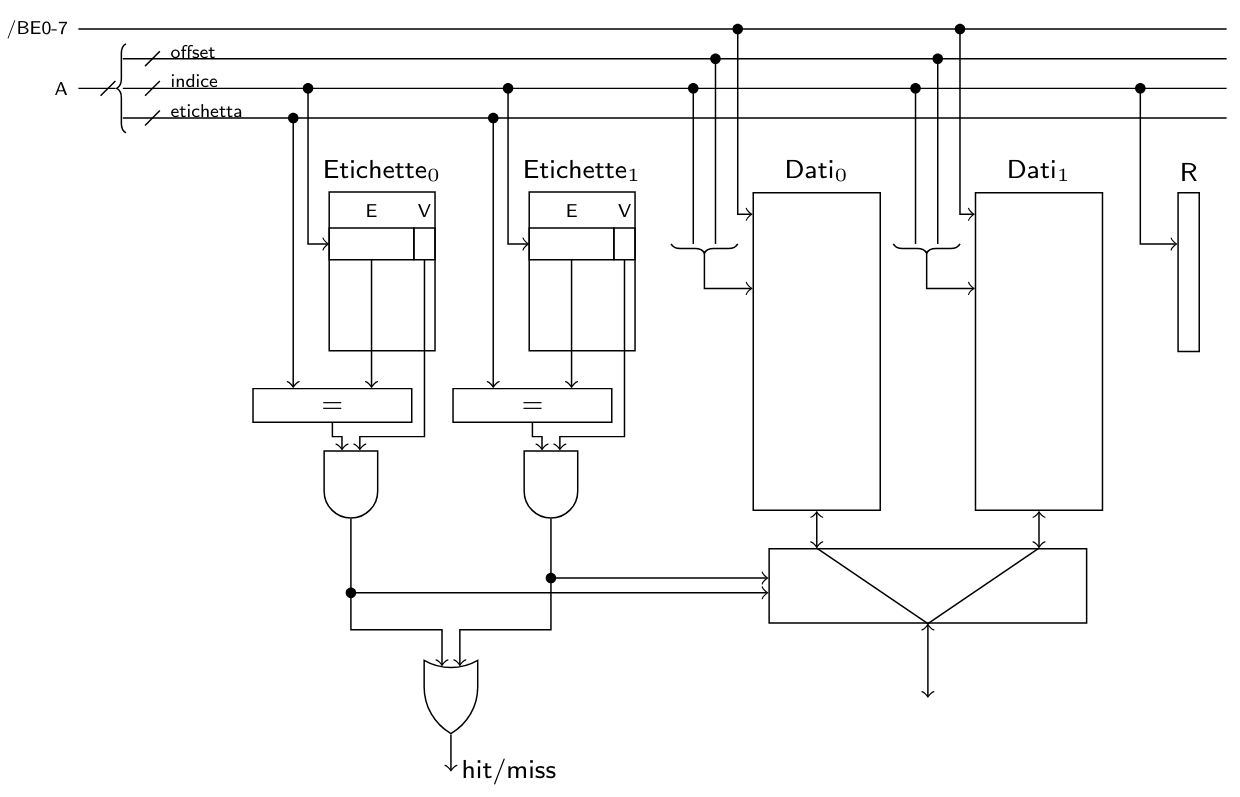
\includegraphics[scale = 0.455]{../figures/cache_associativa.png}
\end{center}

In questo caso a letture allo stesso indice le cache potranno rispondere diversamente (magari la prima in miss e la seconda in hit), e il processore vedrà ritornarsi il dato corretto (in questo caso quello della seconda).

Compito di scegliere quale cache sfruttare nel caso di collisioni è quello del \textbf{controllore} di cache (nella cache ad indirizzamento diretto non c'era scelta). 
La scelta migliore possibile sarebbe quella di scegliere la cacheline al cui i accederà più tardi nel futuro (per mantenere i dati immediatamente utili nella cache).

Chiaramente, visto che non si può prevedere il futuro (o almeno non lo possono fare né la CPU né il controllore di cache), occorre adottare un euristica.
Una di queste euristiche è la politica \textbf{LRU} (\textit{Least Recently Used}), dove si sceglie la cacheline al quale non si accede da più tempo.

Per realizzare tale politica si sfrutta una memoria, che chiamiamo $R$.
Con solo due vie, basterà memorizzare su $R$ l'ultima via usata, e quella su cui scrivere sarà immediatamente l'altra.

Con più di due vie sarebbe necessario mantenere l'ordine degli accessi, cioè per $n$ vie ricordare informazione necessaria a controllare $n!$ diverse possibilità.
Nella pratica, però, conviene usare politiche approssimate.

\subsubsection{Pseudo-LRU dell'80486}
Vediamo una di queste politiche approssimate, implementata nella cache del processore Intel 486, che gestiva 4 insiemi attraverso 3 bit $b_0$, $b_1$ e $b_2$.
Si usava un albero binario per la selezione di una delle vie, disposto come:
\begin{center}
	\begin{forest}
		[$b_0$, roundstyle
			[$b_1$
				[A, rectstyle]
				[B, rectstyle]
				]
			[$b_2$
				[C, rectstyle]
				[D, rectstyle]
			]
		]	
	\end{forest}
\end{center}
dove i valori 1 sono i rami a destra, viceversa i valori 0 sono i rami a sinistra, e gli $\mathsf{A, B, C, D}$ rappresentano i 4 insiemi associativi.

In fase di rimpiazzamento, si sceglie la via seguendo l'albero.
In fase di accesso, si modificano i $b_i$ in modo da portare la via a cui si è fasso accesso in fondo all'ordinamento che si ottiene visitando l'albero.
L'errore può essere dato dal fatto che la via che si trova nello stesso gruppo della via a cui si è fatto accesso potrebbe trovarsi ad un indice più alto del necessario, visto che si abbassa cumulativamente l'intero gruppo aggiornando $b_0$.

\par\smallskip

Ad oggi, anche per cache più grandi si sfruttano sempre algoritmi ad albero di questo tipo, magari tagliando i rami più bassi per lasciare spazio a scelte completamente casuali.

\subsubsection{Cache ed accessi sequenziali}
Notiamo poi che le memorie cache di questo tipo incontrano sempre difficoltà quando si fanno accessi ciclici ad indici che si ripetono con un modulo con il numero di vie diverso da zero: ad esempio se si leggono ciclicamente 5 indirizzi che corrispondono allo stesso indice, la cache non riuscirà mai a mantenere tutti e 5 in una delle cacheline delle vie, e quindi ogni accesso comporterà un miss.

\subsubsection{Livelli di cache}
Come abbiamo accennato, nei processori moderni si hanno solitamente più livelli di cache (3 o 4), che crescono in dimensioni e associatività più si vanno a disporre "lontano" dal processore e "vicini" alla RAM.
Le cache di livello più basso saranno quindi più veloci ma più piccole, mentre le cache di livelo alto saranno più lente ma più grandi.

Il controllore di cache provvederà a gestire i livelli di cache, effettuando gli accessi controllando a partire dal livello più basso (più veloce) per arrivare al livello più basso, fino alla RAM.

\subsection{Interruzioni}
La limitazione principale del processore studiato finora è che il flusso di controllo è completamente determinato dal programma in esecuzione.
L'\textbf{interruzione} viene introdotta per allontanarsi da questo paradigma e introdurre nel processore la possibilità di gestire \textbf{eventi}.
Infatti, attraverso il meccanismo dell'interruzione, il sistema definisce $e_1, ..., e_n$ di questi eventi, e il programmatore $r_1, ..., r_n$ \textbf{routine} per la loro gestione.
Da qui in poi il processore continua ad eseguire il suo normale flusso di controllo, ma monitorando in qualche modo lo stato di questi eventi.
Nel caso uno degli eventi $e_i$ effettivamente si verifichi, il processore provvederà a sospendere il flusso di controllo attuale e ad eseguire la routine $r_i$.

Un esempio classico dell'utilità di un meccanismo di questo tipo è dato dalle fasi di stampa che avevamo definito per dispositivi come schermi o stampanti: attraverso l'approccio visto finora dovremmo controllare periodicamente un certo registro di stato per verificare la possibilità di scrivere un nuovo dato in un certo registro di buffer.
Questo occupa la CPU con operazioni inutili, che potrebbe saltare se fosse la stampante stessa ad avvertirla di quando è pronta a ricevere un nuovo dato.

L'idea di base è quella di avere una nuova operazione da svolgere in fase di esecuzione di un instruzione da parte della CPU, dopo l'esecuzione dell'istruzione stessa.
Ad esempio, potremmo riportarci un bit di validità, \lstinline|READY|, da parte della stampante, e controllarlo ad ogni istruzione per la chiamata di una routine di stampa, cioè aggiungere la seguente circuiteria:
\begin{center}
	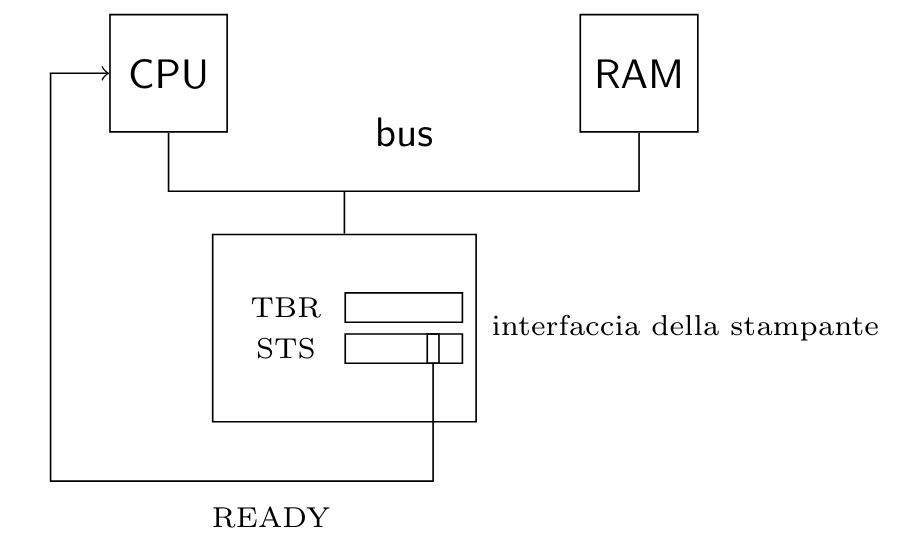
\includegraphics[scale = 0.4]{../figures/int_1.png}
\end{center}

La chiamata sarà semplicemente un aggiornamento condizionato a RIP, con scrittura del contenuto attuale di RIP in pila (che è compatibile con le regole di chiamata dei sottoprogrammi a cui siamo abituati).

Un problema di questo approccio potrebbe essere che, se il bit che segnala l'evento non si aggiorna immediatamente, la CPU andrà in un ciclo continuo di arresto dell'esecuzione e inizio di una routine.
Una soluzione potrebbe essere dotare la CPU di una \textit{rete di accettazione} della rihiesta: il bit di segnalazione dell'evento va in un generatore di impulsi che setta un SR flip-flop, cioè aggiungere la seguente circuiteria:
\begin{center}
	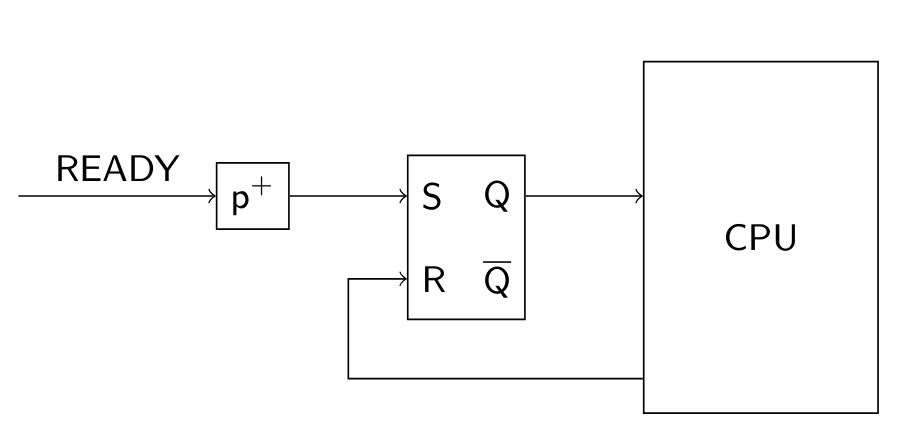
\includegraphics[scale = 0.35]{../figures/int_2.png}
\end{center}

A questo punto la CPU può rispondere (livello hardware, nella nuova fase di esecuzione appena descritta) con un segnale di reset nel momento in cui riesce a rilevare l'evento e spostarsi nella routine. 

In verità la situazione è più complicata: ad esempio potremmo voler ignorare nuovi eventi quando stiamo già cercando di soddisfarne uno.
Per questo i processori x86 prevedono un apposito flag, il flag \textbf{IF} (\textit{Interruption Flag}), che determina se le nuove interruzioni dovranno essere soddisfatte o meno.
Il processore può essere quindi configurato per attivare automaticamente il flag IF in fase di risposta ad una richiesta di interruzione.
Per effettuare il corretto ritorno, si usa la funzione \lstinline|IRETQ|, che ripristina, oltre ad altre cose, lo stato dei flag (che era stato salvato in pila).

Inoltre, probabilmente vorremo gestire più di un interruzione.
Per fare ciò, il processore supporta più tipi di interruzioni, codificati su 8 bit (per un totale di 256 tipi di interruzione).
Vedremo che i primi 32 di questi sono riservati alle cosiddette \textit{eccezioni}, mentre i successivi 224 sono disponibili al programmatore.
Il codice da mandare in esecuzione (nel caso più banale, il semplice valore di RIP da inserire) per ogni interruzione viene mantenuto in una certa struttura dati in memoria, che viene detta \textbf{IVT}, \textit{Interrupt Vector Table}, in modalità reale, e \textbf{IDT}, \textit{Interrupt Descriptor Table}, in modalità protetta.

Abbiamo quindi che il meccanismo delle interruzioni, per citare Dijkstra, \textit{"apre un vaso di pandora"} all'interno dell'architettura dei calcolatori.
Infatti, la loro utilità ha fatto sì che esse non venissero usate solo per l'I/O, ma anche per altre applicazioni.
Possiamo infatti distinguere i tipi di interruzione:
\begin{itemize}
	\item \textbf{Esterne}, quelle introdotte adesso, che come vedremo si dividono a loro volta in \textit{mascherabili} e \textit{non mascherabili};
	\item \textbf{Software}, lanciate dal processore stesso attraverso l'istruzione \lstinline|INT|;
	\item \textbf{Interne} (\textit{eccezioni}), lanciate sempre dal processorein caso di errori ad esso interni.
\end{itemize}

Vediamo l'esempio basilare di un'interruzione software (per noi analoga, almeno per adesso, alle altre 2 in funzionamento), per osservare il funzionamento del meccanismo di interruzione sopratutto riguardo alla pila.
Scriviamo un breve programma misto C++/assembly, di cui la parte C++:
\lstset{style=codestyle, language=C++}
\lstinputlisting{../code/interrupts/sw_basic/main.cpp}
e la parte assembly:
\lstset{style=codestyle, language=assembler}
\lstinputlisting{../code/interrupts/sw_basic/main.s}

Questo tipo di programmazione mista si rende necessario in quanto la gestione dell'interruzione richiede meccanismi accessibili solo all'assembly (in particolare la \lstinline|IRETQ|, che serve per ritornare dal gestore di interruzione).

Ignoriamo quindi per adesso la riga 11 della funzione \lstinline|main()|, che ha il solo compito di impostare il gestore di interruzione per l'interruzione \lstinline|0x40|, e vediamo cosa accade alla riga \lstinline|14|, dove si solleva effettivamente l'interruzione.
In questo caso, il processore sospende l'esecuzione del programma e salta alla funzione \lstinline|a_handler()|, che provvede a salvare i registri, stampare un messaggio, ricaricare i registri e ritornare.
Il contenuto della pila al momento della chiamata di \lstinline|a_handler()| sarà il seguente:
\begin{table}[h!]
	\center
	\begin{tabular} { c | p{9cm} }
		\lstinline|0x20a208| & RIP (main alla riga 15) \\
		\lstinline|0x20a210| & Riservato (CS, per adesso non significativo) \\
		\lstinline|0x20a218| & RFLAGS 
	\end{tabular}
\end{table}

Quindi, come avevamo introdotto, si salva il registro dei flag, un valore per adesso non significativo, e il puntatore corrente (in particolare, quello all'istruzione successiva alla \lstinline|INT|, vedremo significa che si trattava di un interruzione di tipo \textit{trap}).

L'esecuzione del programma dà quindi complessivamente il seguente output:
\begin{lstlisting}[style=shellstyle]
>> sto gestendo l'interruzione                                                                         
>> Premere ESC per proseguire
\end{lstlisting}
cioè siamo riusciti ad interrompere il normale flusso di controllo della funzione \lstinline|main()|, interrompendola a metà esecuzione per eseguire un operazione secondaria, e restituendogli in seguito il normale controllo.

\end{document}
